
\section{shelves and streams}

\begin{frame}{flow model II: shallow shelf approximation (SSA)}
  
SSA model applies very well to \alert{ice shelves}
\begin{itemize}
\item \dots for parts away from grounding lines
\item \dots and away from calving fronts
\end{itemize}

\bigskip

\begin{center}
  \includegraphics[width=0.7\textwidth]{iceshelfedge}

\tiny Ekstr\"om ice shelf (Hans Grobe)
\end{center}
\end{frame}


\begin{frame}{application of SSA to ice streams}

SSA also applies reasonably well to \alert{ice streams}
\begin{itemize}
\item \dots with modest bed topography
\item \dots and weak bed strength\footnote{energy conservation (esp.~ice temperature and basal melt rate) and subglacial hydrology (esp.~subglacial water pressure) are major aspects of ice stream flow \dots but not addressed here!}
\item imperfect near shear margins and grounding lines
\end{itemize}

\begin{center}
  \includegraphics[width=0.5\textwidth]{siple}

\tiny surface velocity for Siple Coast ice streams, Antarctica 
\end{center}
\end{frame}


\begin{frame}{but what is, \emph{and is not}, an ice stream?}

\begin{columns}
\begin{column}{0.4\textwidth}
\includegraphics[width=1.0\textwidth]{streamisbrae}

\bigskip
\scriptsize 
Jakobshavns Isbrae (\textbf{a}) and Whillans Ice Stream (\textbf{b}); plotted without vertical exaggeration (\tiny Truffer and Echelmeyer 2003)\scriptsize)
\end{column}
\begin{column}{0.6\textwidth}
\begin{itemize}
\item[a.] outlet glaciers:
  \begin{itemize}
  \item fast surface speed (up to $10 \,\text{km}\,\text{a}^{-1}$)
  \item uncertain how much is sliding
  \item vertical shear in much of ice column
  \item \emph{not} flat bed topography
  \item soft temperate ice may play big role
  \item \alert{simplifications are dubious}
  \end{itemize}

\medskip
\item[b.] ice streams:
  \small
  \begin{itemize}
  \item fast surface speed (up to $1 \,\text{km}\,\text{a}^{-1}$)
  \item very concentrated vertical shear in thin layer near base (``sliding'')
  \item cold ice nearly down to bed
  \end{itemize}
  \normalsize
\end{itemize}
\end{column}
\end{columns}
\end{frame}


\begin{frame}{SSA stress balance equation}

\begin{itemize}
\item only plane flow case (``flow line'') shown here
\item the stress balance equation, ice stream case:
\begin{empheq}[box=\fbox]{equation}
  \left({\color{red}2 A^{-1/n} H |u_x|^{1/n - 1} u_x}\right)_x - {\color{blue}C|u|^{m-1}u} = {\color{green}\rho g H h_x} \label{ssa}
\end{empheq}
\item the {\color{red} red term} inside parentheses is the vertically-integrated ``longitudinal'' or ``membrane'' stress
\item the {\color{blue} blue term} is basal resistance; $C=0$ in ice shelf
\item the {\color{green} green term} is  driving stress

\medskip
\item this equation determines velocity $u$
\item derived originally by Morland (1987), MacAyeal (1989)
\end{itemize}

\bigskip
\noindent once again, good questions:
\begin{enumerate}
\item[] how to solve (2) numerically?
\item[] how to \emph{think} about it?
\end{enumerate}
\end{frame}


\begin{frame}{flotation criterion and grounding line}

\begin{itemize}
\item the inequality ``$\rho H < - \rho_w b$'' is the \alert{flotation criterion}
  \begin{itemize}
  \item[$\circ$] assumes $z=0$ is sea level
  \item[$\circ$] grounding line $x=x_g$ is where $\rho H = - \rho_w b$
  \item[$\circ$] $H,u,u_x$ are all continuous at $x=x_g$
  \end{itemize}
\item surface elevation and driving stress according to flotation:
  \begin{itemize}
  \item[grounded:]
\begin{align*}
\rho H &> - \rho_w b \\
h &= H + b \\
\rho g H h_x &= \rho g H (H_x + b_x)
\end{align*}
  \item[floating:]
\begin{align*}
\rho H &< - \rho_w b \\
h &= (1-\rho/\rho_w) H \\
\rho g H h_x &= \rho(1-\rho/\rho_w) g H H_x
\end{align*}  
  \end{itemize}
\end{itemize}
\end{frame}


\begin{frame}{flow line model: from stream to shelf}
\label{slide:streamtoshelf}

\small
\begin{align*}
  u = u_0 & \qquad \text{ at } x = 0 \\
  \left.\begin{array}{r}
  \left(2 A^{-1/n} H |u_x|^{1/n - 1} u_x\right)_x - C|u|^{m-1}u = \rho g H h_x \\
  h = H + b
  \end{array}\right\}& \qquad \text{ on } 0 < x < x_g \\
  \left.\begin{array}{r}
  \left(2 A^{-1/n} H |u_x|^{1/n - 1} u_x\right)_x + 0 = \rho g H h_x \\
  h = (1-\rho/\rho_w) H
  \end{array}\right\}& \qquad \text{ on } x_g < x < x_c \\
  2 A^{-1/n} H |u_x|^{1/n - 1} u_x = \frac{1}{2}\rho (1-\rho/\rho_w) g H^2 & \qquad \text{ at } x = x_c
\end{align*}

\bigskip\bigskip
\begin{center}
  \includegraphics[width=0.7\textwidth]{flowline}
\end{center}
\end{frame}


\begin{frame}{steady ice shelf}

\begin{itemize}
\item I have limited goal here:

\begin{center}
\alert{describe a steady state, 1D ice shelf}
\end{center}
\item \emph{by-hand} result (van der Veen 1983): steady SSA ice shelf found from thickness $H_g$ and velocity $u_g$ at the grounding line
   \begin{itemize}
   \item[$\circ$] plots of the exact formulas:

\begin{center}
  \includegraphics[width=0.35\textwidth]{steadyshelfprofile} \qquad \qquad
  \includegraphics[width=0.35\textwidth]{steadyshelfvelocity}
\end{center}

\vspace{-2mm}
   \item[$\circ$] an ice shelf is a kind of fluid \emph{jet}

   \hfill \includegraphics[width=0.3\textwidth]{rocket-nozzle-expansion}
   \end{itemize}

\vspace{-9mm}
\item we will use this to
  \begin{itemize}
  \item[$\circ$] understand the SSA better
  \item[$\circ$] verify a numerical SSA code
  \end{itemize}
\end{itemize}
\end{frame}


\begin{frame}{numerical SSA stress balance example}

I will:
\begin{itemize}
\item fix the ice thickness $H(x)$ from the exact formula
\item find the velocity numerically
\item describe the numerical method for a shelf \emph{or} stream
\item only give a code for an ice shelf
\end{itemize}
\end{frame}


\begin{frame}{numerics of SSA stress balance}

\begin{itemize}
\item the stress balance is a nonlinear equation in the velocity:
  $$\left(2 A^{-1/n} H |u_x|^{1/n - 1} u_x\right)_x - C|u|^{m-1}u = \rho g H h_x$$

\vspace{-2mm}
    \begin{itemize}
    \item[$\circ$] thus \alert{iteration is needed}    
    \end{itemize}
\item coefficient ${\color{red} \bar \nu} = A^{-1/n} |u_x|^{1/n-1}$ is the ``effective viscosity'':
   $$\left(2 \,{\color{red} \bar \nu}\, H u_x\right)_x - C |u|^{m-1} u = \rho g H h_x$$
\item \emph{simplest iteration idea}: use old $\bar\nu$ to get new velocity solution, and repeat until things stop changing
  \begin{itemize}
  \item[$\circ$] this is ``Picard'' iteration  (Newton iteration generally superior)
  \item[$\circ$] from last iterate $u^{(k-1)}$ define
     $$W^{(k-1)} = 2 \bar \nu H = 2 A^{-1/n} |u^{(k-1)}_x|^{1/n-1} H$$
  \item[$\circ$] solve for current iterate $u^{(k)}$:
     $$\left(W^{(k-1)} u^{(k)}_x\right)_x - C |u^{(k-1)}|^{m-1} u^{(k)} = \rho g H h_x$$
  \end{itemize}
\end{itemize}
\end{frame}


\begin{frame}{where do you get an initial guess $u^{(0)}$?}

\begin{itemize}
\item \emph{for floating ice}, assume a uniform strain rate:
   $$u^{(0)}(x) = u_g + \gamma (x-x_g)$$
\item \emph{for grounded ice}, assume ice is held by basal resistance only:
   $$u^{(0)}(x) = \left(-C^{-1} \rho g H h_x\right)^{1/m}$$
\end{itemize}
\end{frame}


\begin{frame}{abstract the ``inner'' linear problem}
\begin{itemize}
\item abstract problem:
   $$\left(W(x)\, u_x\right)_x - \alpha(x)\, u = \beta(x)$$

\vspace{-2mm}
  \begin{itemize}
  \item[$\circ$] on $0 < x < L$
  \item[$\circ$] at grounding line $x_g=0$: \quad $u(0) = u_g$
  \item[$\circ$] at calving front $x_c=L$: \quad\,\, $u_x(L) = \gamma$
  \end{itemize}
\item an \emph{elliptic} boundary value problem
\item $W(x)$, $\alpha(x)$, $\beta(x)$ are known functions in the SSA context:
  \begin{itemize}
  \item[$\circ$] both $W(x)$ and $\alpha(x)$ come from previous iteration
  \item[$\circ$] $\beta(x)$ is driving stress
  \end{itemize}
\end{itemize}
\end{frame}


\begin{frame}{numerics of the ``inner'' linear problem}

\begin{itemize}
\item suppose $j=1,2,\dots,J+1$, where $x_1 = x_g$ and $x_{J+1} = x_c$ are endpoints
\item $W(x)$ is needed on the staggered grid; the approximation is:
$$\frac{W_{j+1/2} (u_{j+1} - u_j) - W_{j-1/2} (u_{j} - u_{j-1})}{\Delta x^2} - \alpha_j u_j \stackrel{\ast}{=} \beta_j$$
\item left-hand boundary condition: $u_1 = u_g$ given
\item right-hand boundary condition:
  \begin{itemize}
  \item[$\circ$] introduce notional point $x_{J+2}$
  \item[$\circ$] approximate ``$u_x(L)=\gamma$'' by
    $$\frac{u_{J+2} - u_J}{2 \Delta x} = \gamma$$
  \item[$\circ$] use $j=J+1$ case of $\ast$ to eliminate $u_{J+2}$ (by-hand)
  \end{itemize}
\end{itemize}
\end{frame}


\begin{frame}{numerics of the ``inner'' linear problem 2}

\footnotesize
\begin{itemize}
\item thus iterate of SSA stress balance has form  \quad $A \mathbf{x} = \mathbf{b}$:
$$
\begin{bmatrix}
1 &  &  &  &  \\
W_{3/2} & A_{22} & W_{5/2} &  &  \\
 & W_{5/2} & A_{33} &  &  \\
 &  & \ddots & \ddots &  \\
 &  & W_{J-1/2} & A_{JJ} & W_{J+1/2} \\
 &  &  & A_{J+1,J} & A_{J+1,J+1} \\
\end{bmatrix}\,
\begin{bmatrix}
u_1 \\ u_2 \\ u_3 \\ \vdots \\ u_J \\ u_{J+1}
\end{bmatrix}
=
\begin{bmatrix}
u_g \\ \beta_2 \Delta x^2 \\ \beta_3 \Delta x^2 \\ \vdots \\ \beta_J \Delta x^2 \\ b_{J+1}
\end{bmatrix}
$$
\item diagonal entries
$$A_{22} = -(W_{3/2}+W_{5/2}+\alpha_1 \Delta x^2), \quad A_{33} = -(W_{5/2}+W_{7/2}+\alpha_2 \Delta x^2), \quad \dots$$
\item special cases in final equation:
$$A_{J+1,J} = 2 W_{J+1/2}$$
$$A_{J+1,J+1} = -(2 W_{J+1/2}+\alpha_{J+1}\Delta x^2)$$
$$b_{J+1} = -2 \gamma \Delta x W_{J+3/2} + \beta_{J+1} \Delta x^2$$
\item this is a \emph{tridiagonal} system
\end{itemize}
\end{frame}


\begin{frame}{numerics of the ``inner'' linear problem 3}
\label{slide:flowlinecode}

\minput{flowline}
\end{frame}


\begin{frame}{testing the abstracted linear code}

\begin{itemize}
\item first we test the linear code \texttt{flowline.m} for the abstract problem
\item test by ``manufacturing'' solutions
  \begin{itemize}
  \item[$\circ$] see \texttt{testflowline.m}
  \item[$\circ$] result: converges at optimal rate $O(\Delta x^2)$
  \end{itemize}

\bigskip
\item then write Picard iteration loop to create SSA nonlinear solver
  \begin{itemize}
  \item[$\circ$] \texttt{ssaflowline.m} on next slide
  \end{itemize}
\end{itemize}
\end{frame}


\begin{frame}{numerical SSA implementation}

\minputtiny{ssaflowline}
\end{frame}


\begin{frame}{numerical convergence}

convergence analysis of \texttt{ssaflowline.m}:

\begin{center}
  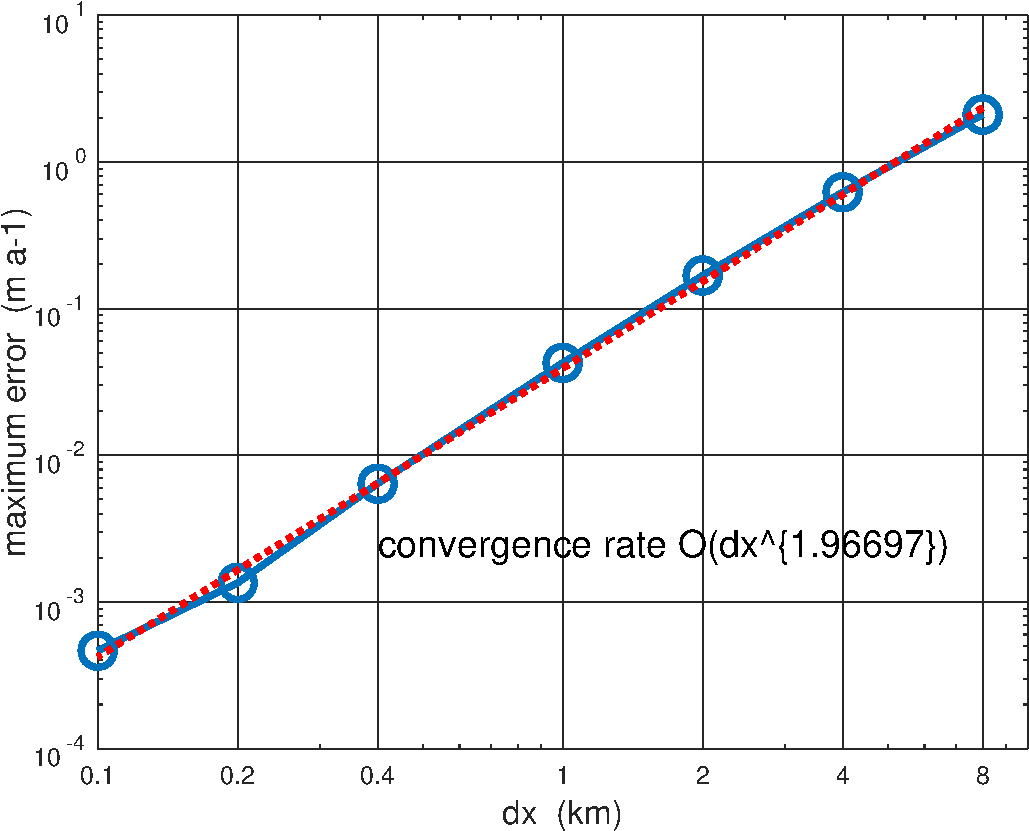
\includegraphics[width=0.75\textwidth]{shelfconv}
\end{center}
\end{frame}


\begin{frame}{SSA numerical model output}

\begin{center}
  \includegraphics[width=0.45\textwidth]{steadyshelfprofile} \quad
  \includegraphics[width=0.45\textwidth]{steadyshelfvelocity}
\end{center}

\bigskip

\begin{itemize}
\item \emph{this looks suspiciously like figures for the exact solution \dots}
\item yes
\end{itemize}
\end{frame}

\begin{frame}{numerical ice shelf modeling in 2D}

\begin{itemize}
\item flow lines are never very realistic
  \begin{itemize}
  \item[$\circ$] you can add parameterized ``side drag''
  \end{itemize}
\item ``diagnostic'' (static geometry) ice shelf modeling in 2d has been quite successful
\item observed surface velocities validate SSA stress balance model
  \begin{itemize}
  \item[$\circ$] e.g.~Ross ice shelf example below using PISM
  \item[$\circ$] \dots many models can do this
  \end{itemize}
\end{itemize}

\begin{center}
\includegraphics[width=0.45\textwidth]{rossquiver}  \hfill  \includegraphics[width=0.45\textwidth]{rossscatter}
\end{center}
\end{frame}


\begin{frame}{numerical solution of stress balances: a summary}

\begin{itemize}
\item stress balance equations (e.g.~SSA or Stokes) determine velocity from geometry and boundary conditions
\item for ice the equations are nonlinear so iteration is necessary
  \begin{itemize}
  \item[$\circ$] at each iteration a sparse matrix ``inner'' problem is solved
  \item[$\circ$] give it to a linear algebra package; don't write it yourself
  \end{itemize}
\item when geometry and boundary stresses are \emph{known}, many modern stress balance solvers do well
  \begin{itemize}
  \item[$\circ$] e.g.~ice shelves
  \item[$\circ$] model shallowness often is \emph{not} the issue
  \item[$\circ$] see: Aschwanden et al.~(2016), \emph{Complex Greenland outlet glacier flow captured}
  \end{itemize}
\end{itemize}
\end{frame}


\section{free advice}

\begin{frame}{best practices for numerical modeling}

\begin{itemize}
\item learn a version-control system \hfill \alert{\texttt{git}}
\item put your project on a public host from the beginning
  \begin{itemize}
  \item[$\circ$] to hell with your secretive advisor \hfill \alert{\texttt{github.com}}
  \end{itemize}
\item modularize your codes
\item test the parts
  \begin{itemize}
  \item[$\circ$] make testing easily repeatable \hfill \alert{\texttt{make test}}
  \end{itemize}
\item if you are stuck:
  \begin{itemize}
  \item[$\circ$] write documentation for what you have
  \item[$\circ$] go find exact solutions and literature about submodels
  \end{itemize}
\end{itemize}
\end{frame}


\begin{frame}{}
\begin{itemize}
\item this thing

\vspace{-10mm}
\begin{center}

\includegraphics[width=0.5\textwidth]{computer}
\end{center}
\alert{does not know what you \emph{intend}}, your physical modelling goal
   \begin{itemize}
   \item[$\circ$] it does ``know'' your discrete equations, the program you wrote
   \end{itemize}

\bigskip
\item you \emph{can} aspire for your computer to ``know'' your continuum model, the one that you write as PDEs
   \begin{itemize}
   \item[$\circ$] achieve this through verification with exact solutions
   \end{itemize}
\end{itemize}

\end{frame}
